% Author Name: José António Portela Areia
% Author Contact: jose.apareia@gmail.com
% Version: 2.2.5 - 2025/03/15
% Public Repository: https://github.com/joseareia/ipleiria-thesis
% Wiki/Getting Help: https://github.com/joseareia/ipleiria-thesis/wiki

%%% Document Options %%%
\documentclass[
    language=english,
    school=estg,
    docstage=final,
    media=paper,
    linkcolor=red!45!black,
    chapterstyle=classic,
    coverstyle=classic
]{OkraThesis} % Refer to the Wiki for a list of available options.

%%% Document Version %%%
\DocumentVersion{1.0.0} % This is required only if the 'docstage' is set to 'working'.

%%% Document Metadata %%%
% First Author (Mandatory)
\FirstAuthor{Edun Joshua}
\FirstAuthorNumber{2230455}

% Second Author (Optional)
\SecondAuthor{Mbuotidem Awak}
\SecondAuthorNumber{2230456}

% Third Author (Optional)
\ThirdAuthor{Makinde Kayode}
\ThirdAuthorNumber{2230457}

% Supervisor (Mandatory)
\Supervisor{Data Community Africa, AgriConnect, Dicey Tech, REDtech Africa}
\SupervisorMail{joe.smith@ipleiria.pt}
% Please provide: [Current Title, Affiliation]
\SupervisorTitle{Full Professor, Polytechnic of Leiria} 

% Co-Supervisor (Optional)
\CoSupervisor{Steve Smith}
\CoSupervisorMail{steve.smith@ipleiria.pt}
\CoSupervisorTitle{Associate Professor, Polytechnic of Leiria}

% Second Co-Supervisor (Optional)
\SecCoSupervisor{Shak Smith}
\SecCoSupervisorMail{shak.smith@ipleiria.pt}
\SecCoSupervisorTitle{Associate Researcher, Computer Science \& Communication Research Centre}

% Title (Mandatory)
\Title{Post-Harvest Losses Problem: Reducing Post-Harvest Losses to Build Youth-Led Agri-Businesses}

% Subtitle (Mandatory)
\Subtitle{Investigating Strategies to Mitigate PHL}

% University (Mandatory)
\University{Polytechnic of Leiria}

% School (Mandatory)
\School{Data Community Africa}

% Department (Mandatory)
\Department{Department of Computer Engineering}

% Degree (Mandatory)
\Degree{Master in Cybersecurity \& Digital Forensics}

% Course (Optional)
% \Course{Offensive \& Defensive Cybersecurity}

% Thesis Theme (Mandatory)
\ThesisType{Academic report 
% \\ 
% \textcolor{blue}{(Erase the Non-Essential)}
}

% Local & Date (Mandatory)
\Date{Lagos, \DTMmonthname{\month} \number\year}

% Academic Year 
\AcademicYear{2024/25}

%%% Loading of Glossary and Acronyms %%%
\makeglossaries
\loadglsentries{Matter/04-Glossary}
\loadglsentries[\acronymtype]{Matter/05-Acronyms}

\begin{document}

%%% Front Matter %%%
\ifthenelse{\equal{\CoverOption}{classic}}{
    \newcommand\BackgroundPicCover{%
    \put(0,0){%
    \parbox[b][\paperheight]{\paperwidth}{%
    \vfill
    \centering
    \includegraphics[width=\paperwidth,height=\paperheight,keepaspectratio]{Figures/Theme/Cover-BG.pdf}%
    \vfill
    }}}
}{
    \newcommand\BackgroundPicCover{%
    \put(0,0){%
    \parbox[b][\paperheight]{\paperwidth}{%
    \vfill
    \centering
    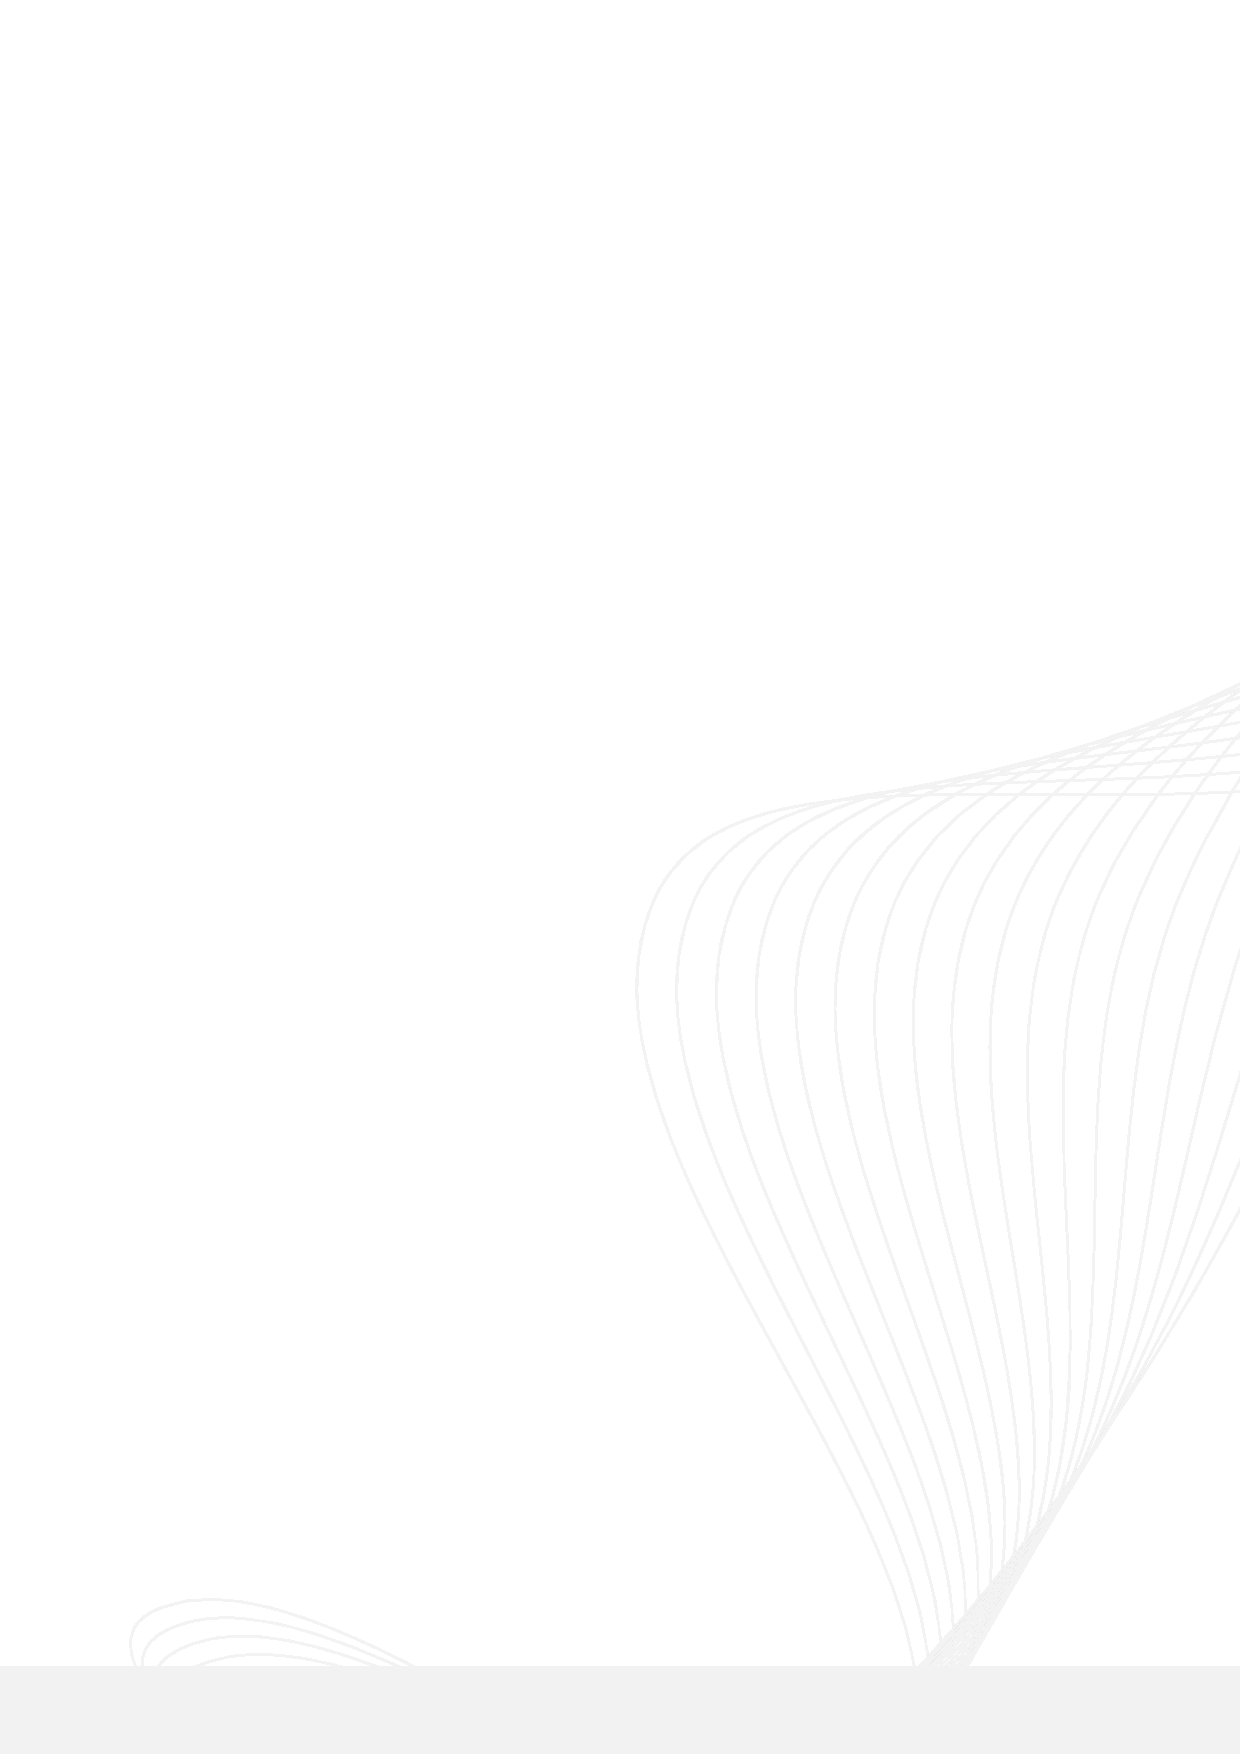
\includegraphics[width=\paperwidth,height=\paperheight,keepaspectratio]{Figures/Theme/Front-Page-BG.pdf}%
    \vfill
    }}}
}

\AddToShipoutPictureBG*{\BackgroundPicCover}

\newgeometry{margin=1.98cm, top=2.15cm, bottom=1.47cm}
\begin{titlepage}
    \latofont
    \ifthenelse{\equal{\CoverOption}{classic}}{\color{white}}{\color{frontpagedark}}
    \vspace*{\baselineskip}

    \ifthenelse{\equal{\CoverOption}{classic}}{
        \ifthenelse{\equal{\SchoolOption}{estg}}{
            % \begin{figure}
            %     
\includegraphics[width=0.485\linewidth]{Figures/Theme/Logotypes/IPLeiria-ESTG-Logo-W.pdf}
            % \end{figure}
        }{}
        
        \ifthenelse{\equal{\SchoolOption}{esad}}{
            % \begin{figure}
            %     
\includegraphics[width=0.485\linewidth]{Figures/Theme/Logotypes/IPLeiria-ESAD-Logo-W.pdf}
            % \end{figure}
        }{}
        
        \ifthenelse{\equal{\SchoolOption}{esslei}}{
            % \begin{figure}
            %     
\includegraphics[width=0.485\linewidth]{Figures/Theme/Logotypes/IPLeiria-ESSLEI-Logo-W.pdf}
            % \end{figure}
        }{}
        
        \ifthenelse{\equal{\SchoolOption}{estm}}{
            % \begin{figure}
            %     
\includegraphics[width=0.485\linewidth]{Figures/Theme/Logotypes/IPLeiria-ESTM-Logo-W.pdf}
            % \end{figure}
        }{}
        
        \ifthenelse{\equal{\SchoolOption}{esecs}}{
            % \begin{figure}
            %     
\includegraphics[width=0.485\linewidth]{Figures/Theme/Logotypes/IPLeiria-ESECS-Logo-W.pdf}
            % \end{figure}
        }{}
    } {
        \ifthenelse{\equal{\SchoolOption}{estg}}{
            \begin{figure}
                
\includegraphics[width=0.485\linewidth]{Figures/Theme/Logotypes/IPLeiria-ESTG-Logo-B.pdf}
                % 
\includegraphics[width=0.4\linewidth]{Figures/Theme/Logotypes/IPLeiria-ESTG-Logo-Old.png}
            \end{figure}
        }{}
        
        \ifthenelse{\equal{\SchoolOption}{esad}}{
            \begin{figure}
                
\includegraphics[width=0.485\linewidth]{Figures/Theme/Logotypes/IPLeiria-ESAD-Logo-B.pdf}
            \end{figure}
        }{}
        
        \ifthenelse{\equal{\SchoolOption}{esslei}}{
            \begin{figure}
                
\includegraphics[width=0.485\linewidth]{Figures/Theme/Logotypes/IPLeiria-ESSLEI-Logo-B.pdf}
            \end{figure}
        }{}
        
        \ifthenelse{\equal{\SchoolOption}{estm}}{
            \begin{figure}
                
\includegraphics[width=0.485\linewidth]{Figures/Theme/Logotypes/IPLeiria-ESTM-Logo-B.pdf}
            \end{figure}
        }{}
        
        \ifthenelse{\equal{\SchoolOption}{esecs}}{
            \begin{figure}
                
\includegraphics[width=0.485\linewidth]{Figures/Theme/Logotypes/IPLeiria-ESECS-Logo-B.pdf}
            \end{figure}
        }{}
    }

    \vspace{5.5\baselineskip}

    % % Title.
	% \noindent
    % \makebox[\textwidth][l]{%
    %     \parbox{\dimexpr\textwidth-4cm\relax}{
    %         \setstretch{1.03}
    %         \raggedright\bfseries\fontsize{20}{26}\selectfont\GetTitle
    %     }
    % }

    \vspace{0.8\baselineskip}

    % Subtitle.
    % \noindent
    % \makebox[\textwidth][l]{%
    %     \parbox{\dimexpr\textwidth-7cm\relax}{
    %         \setstretch{1.03}
    %         \raggedright\fontsize{14}{19}\selectfont\GetSubtitle
    %     }
    % }

    \vspace{35pt}  

    % Author.
    {\noindent\bfseries\fontsize{14}{19}\selectfont\GetFirstAuthor}

    \ifdefined\GetSecondAuthor
        \vspace{8pt}
        {\noindent\bfseries\fontsize{14}{19}\selectfont\GetSecondAuthor}
	\fi

    \ifdefined\GetThirdAuthor
        \vspace{8pt}
        {\noindent\bfseries\fontsize{14}{19}\selectfont\GetThirdAuthor}
	\fi
 
	\vfill

    % % School.
	% {\noindent\fontsize{10}{12}\selectfont\GetSchool}
	
    % % Department.
	% {\noindent\fontsize{10}{12}\selectfont\GetDepartment}

    % % Degree.
	% {\noindent\fontsize{10}{12}\selectfont\GetDegree}

    % Course.
    \ifdefined\GetCourse
        {\noindent\fontsize{10}{12}\selectfont\GetCourse}
	\fi

    \ifthenelse{\equal{\DocStageOption}{working}}{
        \vspace{62pt}
        {\noindent\fontsize{10}{12}\selectfont\overwritecolor{yellow}{\GetDocumentVersion \\ \textit{\today}}} 
        \vspace{62pt}
    }{
        \vspace{125pt}
    }

    % Local & Date.
	{\noindent\fontsize{10}{12}\selectfont\GetDate}

    \vspace{68pt}
\end{titlepage}
\restoregeometry
\MediaOptionLogicBlank
\newcommand\BackgroundPicFrontPage{%
    \put(0,0){%
    \parbox[b][\paperheight]{\paperwidth}{%
    \vfill
    \centering
    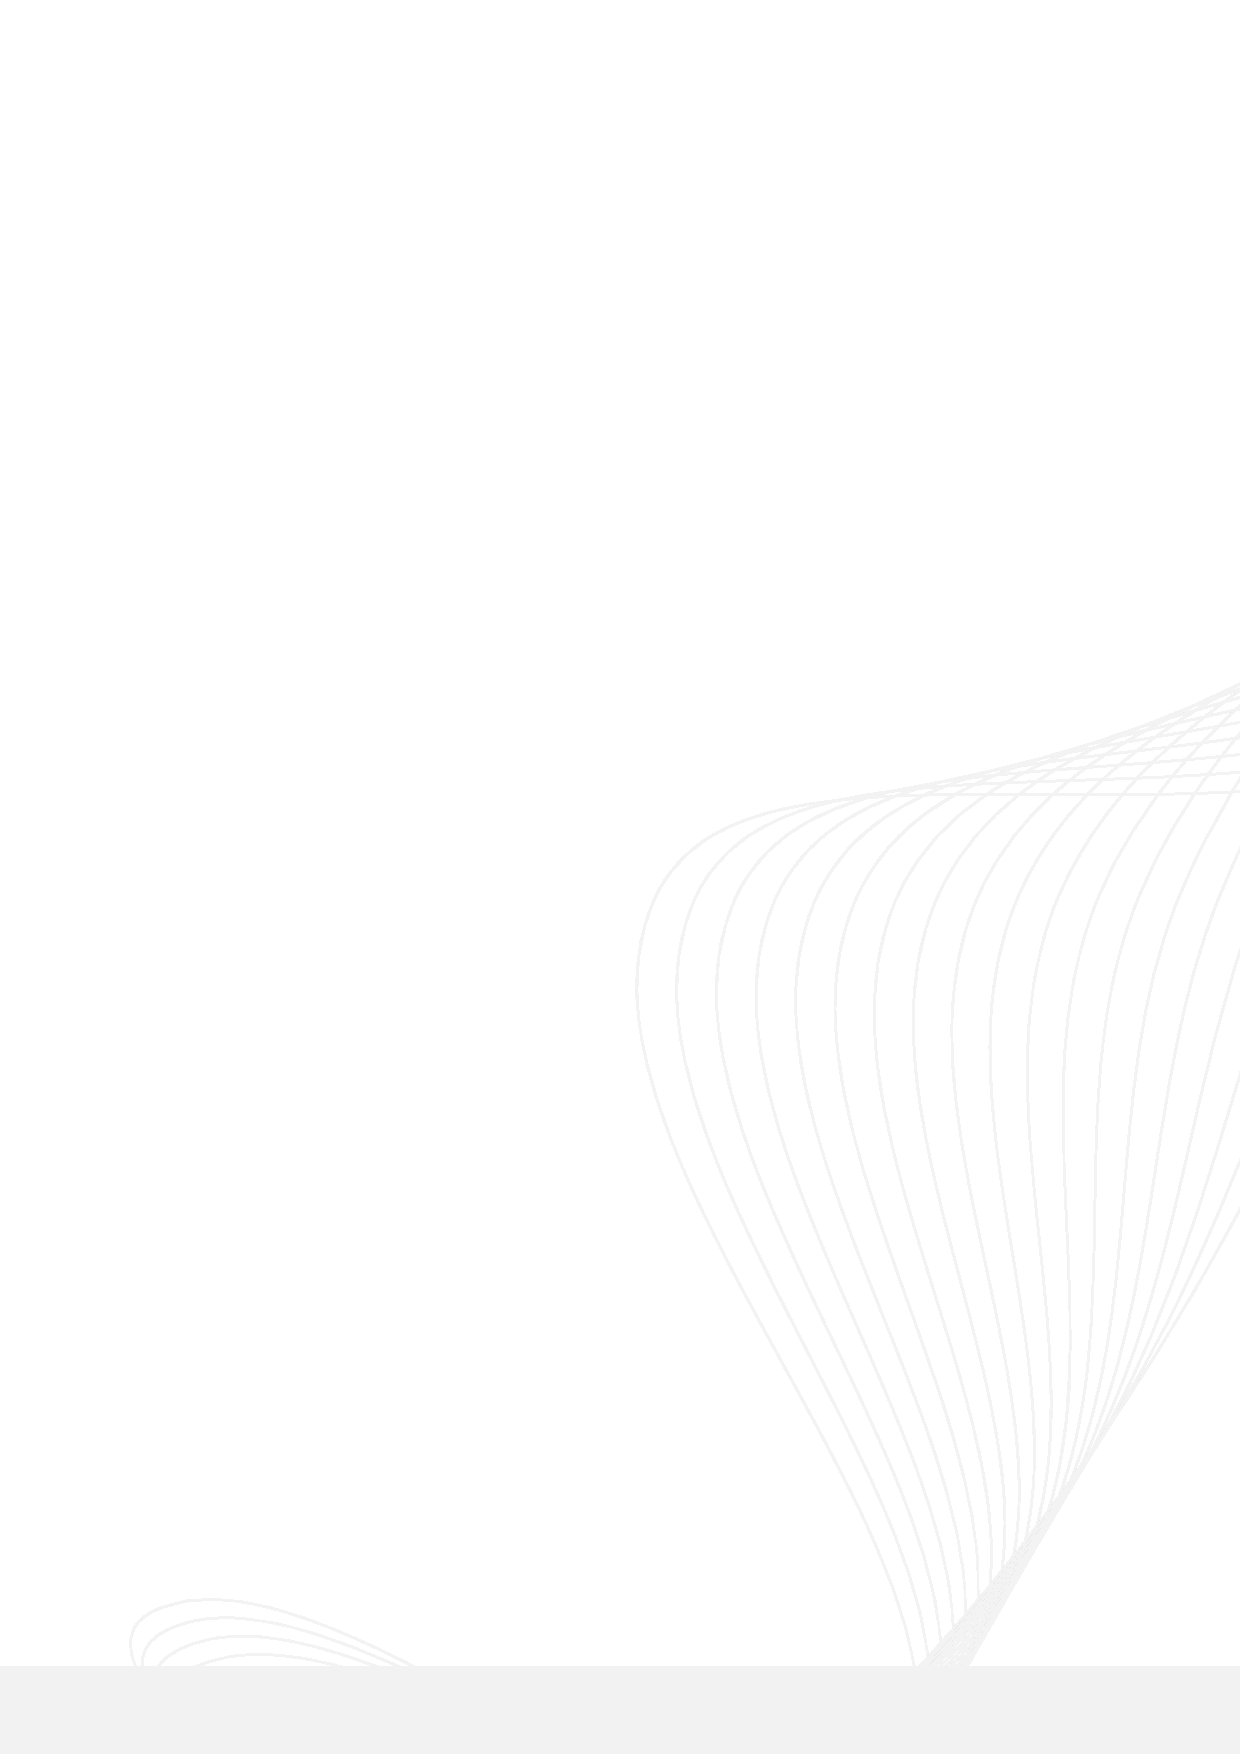
\includegraphics[width=\paperwidth,height=\paperheight,keepaspectratio]{Figures/Theme/Front-Page-BG.pdf}%
    \vfill
}}}
\AddToShipoutPictureBG*{\BackgroundPicFrontPage}

\newgeometry{margin=1.98cm, top=2.15cm, bottom=1cm}
\begin{titlepage}
    \latofont
    \color{frontpagedark}
    \vspace*{\baselineskip}

    \ifthenelse{\equal{\SchoolOption}{estg}}{
        \begin{figure}
            
\includegraphics[width=0.485\linewidth]{Figures/Theme/Logotypes/logo-green.pdf}
            % 
\includegraphics[width=0.4\linewidth]{Figures/Theme/Logotypes/IPLeiria-ESTG-Logo-Old.png}
        \end{figure}
    }
    
    \ifthenelse{\equal{\SchoolOption}{esad}}{
        \begin{figure}
            
\includegraphics[width=0.485\linewidth]{Figures/Theme/Logotypes/IPLeiria-ESAD-Logo-B.pdf}
        \end{figure}
    }
    
    \ifthenelse{\equal{\SchoolOption}{esslei}}{
        \begin{figure}
            
\includegraphics[width=0.485\linewidth]{Figures/Theme/Logotypes/IPLeiria-ESSLEI-Logo-B.pdf}
        \end{figure}
    }
    
    \ifthenelse{\equal{\SchoolOption}{estm}}{
        \begin{figure}
            
\includegraphics[width=0.485\linewidth]{Figures/Theme/Logotypes/IPLeiria-ESTM-Logo-B.pdf}
        \end{figure}
    }
    
    \ifthenelse{\equal{\SchoolOption}{esecs}}{
        \begin{figure}
            
\includegraphics[width=0.485\linewidth]{Figures/Theme/Logotypes/IPLeiria-ESECS-Logo-B.pdf}
        \end{figure}
    }

    \vspace{3.5\baselineskip}

    % Title.
	\noindent
    \makebox[\textwidth][l]{%
        \parbox{\dimexpr\textwidth-2.5cm\relax}{
            \setstretch{1.03}
            \raggedright\bfseries\fontsize{20}{26}\selectfont\GetTitle
        }
    }

    \vspace{0.8\baselineskip}

    % Subtitle.
    \noindent
    \makebox[\textwidth][l]{%
        \parbox{\dimexpr\textwidth-7cm\relax}{
            \setstretch{1.03}
            \raggedright\fontsize{14}{19}\selectfont\GetSubtitle
        }
    }

    \vspace{35pt}

    % Author.
    {\noindent\bfseries\fontsize{14}{19}\selectfont\GetFirstAuthor}

    \ifdefined\GetSecondAuthor
        \vspace{8pt}
        {\noindent\bfseries\fontsize{14}{19}\selectfont\GetSecondAuthor}
	\fi

    \ifdefined\GetThirdAuthor
        \vspace{8pt}
        {\noindent\bfseries\fontsize{14}{19}\selectfont\GetThirdAuthor}
	\fi

    \vspace{70pt}    

    {
    \noindent
    \latofont
    \fontsize{10}{12}\selectfont
    \renewcommand{\arraystretch}{0.1}
    \hspace*{-2.5pt}\begin{tabular}{@{}r@{\hspace{5pt}}>{\raggedright\arraybackslash}m{6cm}@{}}
        \textbf{Organizers:} & \GetSupervisor \\ [-.7ex]
        % & \setstretch{0.9}{\fontsize{8}{10}\selectfont\itshape \GetSupervisorTitle} \\ [2ex]
        
        % \ifdefined\GetCoSupervisor
        %     \textbf{Co-supervisor:} & \GetCoSupervisor \\ [-.7ex]
        %     & \setstretch{0.9}{\fontsize{8}{10}\selectfont\itshape \GetCoSupervisorTitle} \\ [.5ex]
        % \fi

        % \ifdefined\GetSecCoSupervisor        
        %     & \GetSecCoSupervisor \\ [-.7ex]
        %     & \setstretch{0.9}{\fontsize{8}{10}\selectfont\itshape \GetSecCoSupervisorTitle} \\
        % \fi
    \end{tabular}
    }
    
    \vfill
	
    % School.
	% {\noindent\fontsize{10}{12}\selectfont\GetSchool}
	
    % % Department.
	% {\noindent\fontsize{10}{12}\selectfont\GetDepartment}

    % % Degree.
	% {\noindent\fontsize{10}{12}\selectfont\GetDegree}

    % Course.
    % \ifdefined\GetCourse
    %     {\noindent\fontsize{10}{12}\selectfont\GetCourse}
	% \fi

    \vspace{20pt}

    % Thesis option.
	{\noindent\fontsize{10}{12}\itshape\selectfont\GetThesisType}

    \vspace{20pt}

    % Local and date.
	{\noindent\fontsize{10}{12}\selectfont\GetDate}

    \vspace{68pt}
\end{titlepage}
\restoregeometry
\MediaOptionLogicBlank

%%% Copyright Statement %%%
\pagenumbering{gobble} % Prevent page numbering.

\vspace*{\fill}

\ifthenelse{\equal{\LanguageOption}{portuguese}}{%
    \noindent \textbf{\GetTitle}
    
    \noindent Copyright \textcopyright~\the\year{} - \GetFirstAuthor, \GetSecondAuthor, \GetThirdAuthor; \GetSchool.
    
    \vspace{.575em}
    
    \noindent This dissertation is original work, written solely for this purpose, and all the authors whose studies and publications contributed to it have been duly cited. Partial reproduction is allowed with acknowledgment of the author and reference to the year, institution - \textit{Data Community Africa} - and public defense date.
}{%
    \noindent \textbf{\GetTitle}
    
    \noindent Copyright \textcopyright~\the\year{} - \GetFirstAuthor, \GetSchool.
    
    \vspace{.575em}
    
    \noindent This dissertation is original work, written solely for this purpose, and all the authors whose studies and publications contributed to it have been duly cited. Partial reproduction is allowed with acknowledgment of the author and reference to the year, institution - \textit{Data Community Africa} - and public defense date.
}

\vspace*{\fill}
\MediaOptionLogic

%%% Roman Numeration %%%
\pagenumbering{roman}

%%% Acknowledgements %%%
\ifthenelse{\equal{\LanguageOption}{portuguese}}{%
    \chapter*{Agradecimentos}
}{%
    \chapter*{Acknowledgements}
}

% \guideinfo{In the \textit{Acknowledgment} section, express your gratitude to those who helped and supported your work. Start by thanking your advisors, mentors, or supervisors who provided guidance and expertise. Mention any colleagues, classmates, or team members who contributed to discussions or offered assistance. You can also acknowledge specific organisations, institutions, or funding sources that supported your research or work. Lastly, include any personal acknowledgments for family or friends who offered encouragement and moral support during the project. Keep this section sincere, concise, and professional.}

{Our deepest thanks go to the \href{https://www.linkedin.com/company/datafestafrica/}{Data Community Africa} community. We attribute significant professional growth to the foundation and resources they consistently provide.
\vspace{\myvspace}

We are also immensely grateful to \href{https://www.linkedin.com/company/redtech-africa/}{REDTech} and DiceyTech \href{https://www.linkedin.com/company/diceytech/}{DiceyTech} for sponsoring valuable hackathons like this. They empower data enthusiasts by offering crucial opportunities to challenge themselves and showcase their abilities.}

\MediaOptionLogicBlank

%%% Abstract %%%
\thispagestyle{plain}
% \chapter*{Resumo}

% \guiainfo{Na secção \textit{Resumo}, apresente um resumo conciso do seu projeto, destacando os pontos principais. Comece com uma breve declaração do problema ou objetivo, seguido de uma descrição da sua abordagem ou metodologia. Resuma os principais resultados ou conclusões, salientando a sua importância ou implicações. Conclua com uma ou duas frases sobre a contribuição global ou o impacto do seu trabalho. O resumo deve ser claro e conciso, idealmente com 150-250 palavras, para que os leitores compreendam rapidamente o seu trabalho e a sua importância.}

% \keywordspt{Palavra-Chave A, Palavra-Chave B, Palavra-Chave C.}

%\MediaOptionLogicBlank

\pdfbookmark[1]{Abstract}{abstract}
\chapter*{Abstract}
% \guideinfo{In the \textit{Abstract} section, provide a concise summary of your project, highlighting the key points. Begin with a brief statement of the problem or objective, followed by a description of your approach or methodology. Summarise the main results or findings, emphasising their significance or implications. Conclude with a sentence or two on the overall contribution or impact of your work. Keep the abstract clear and focused, ideally within 150-250 words, to give readers a quick understanding of your research and its importance.}

{In Nigeria, millions of tons of food go to waste every year; not because of poor harvests, but because they never make it from farms to markets. To tackle these losses, we present Okra — a data-driven digital marketplace and logistics platform built to seamlessly connect farmers, buyers, and logistics providers in real time.  Its stand-out feature is an AI-powered tool for predicting freshness and quantity of produce using image recognition, and helping buyers make faster, more informed decisions. Okra also uses data such as rainfall forecasts and harvest schedules to predict high-risk post-harvest loss periods, enabling early interventions like dispatching logistics or alerting farmers.}

\keywordsen{Post Harvest Loss, Digital Marketplace, AI.}

\MediaOptionLogicBlank

%%% Table of Contents, List of Figures and List of Tables %%%
\bookmarktocentry\tableofcontents
\listoffigures
\listoftables

%%% Print: Glossary and Acronyms %%%
\glossarytoc\printnormalglossary
\acronymtoc\printacronymglossary

%%% Arabic Numeration %%%
 \pagenumbering{arabic}

%%% Chapters (**Insert Yours Here**) %%%
\chapter[Introduction]{Introduction}
\label{cp:introduction}

{
\parindent0pt

\textit{Authors: Edun Joshua, Mboutidem Awak, Makinde Kayode}

% \textit{Current Version: 2.2.4}

\textit{License: \LaTeX~Project Public License v1.3c}

\textit{Official Repository: \href{https://github.com/joseareia/ipleiria-thesis}{GitHub Repository}}

\vspace{.935em}

\acrfull{phl} refers to the measurable reduction in the quantity or quality of food after harvest, making it unfit for consumption
 \citep{FAO_PostHarvest}. Globally, roughly one-third of food produced is lost or wasted. In Nigeria, the scope is especially alarming: studies estimate that the country loses on the order of 40–50\% of its total food production each year.



\begin{block}[note]
    \textit{“Each year, Nigeria wastes 40\% of its total food production”, equivalent to significant greenhouse gas emissions
    \citep{worldbank2020}.}
    \end{block}
    


 \section{Analysis of Post-Harvest Losses in Nigeria}   

According to \citet{NAN2024}, FAO experts similarly report losses around 50\% for certain crops. 
USAID reports that post-harvest losses for fresh produce in Nigeria can reach almost 50\% \citet{Udi2024}, and for tubers, fruits, and vegetables, losses can range between 50\% and 60\% \citep{OkojieJaiyesimi2024}.
These statistics reveal a gap between Nigeria’s agricultural output and what actually reaches consumers. \autoref{fig:figure-01} illustrates the estimated post-harvest losses for key crops in Nigeria, according to the APHLIS database \citep{APHLIS}.


\begin{figure}[H]
    \centering
    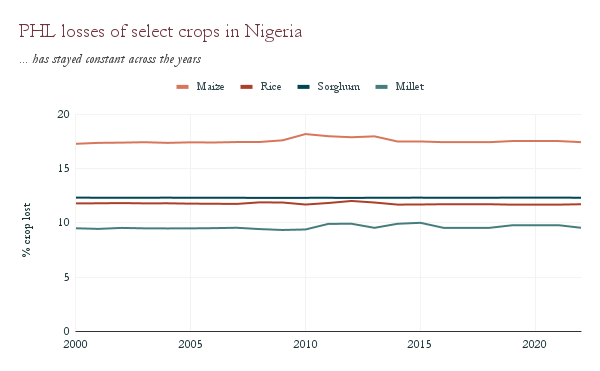
\includegraphics[scale=0.8]{Figures/phl_crops_v2.png}
    \caption{\acrshort{phl} in Nigeria for key crops. Source: APHLIS database, 2019}
    \label{fig:figure-01}
\end{figure}

\autoref{fig:figure-02} shows post-harvest losses across different value chain steps from 2018 to 2022. The total estimated loss peaked in 2019 at over 2.2 million tonnes, followed by slight declines in subsequent years. The highest losses consistently occurred during the harvesting/field drying and household-level storage phases, which together accounted for over half of total losses in all years.
Losses during further drying and threshing and shelling remained moderate but stable across the years. Transport from the field showed smaller but steady losses, while losses during transport to market and market storage were recorded as zero for all years, possibly due to either minimal losses or lack of data collection at those points. These trends suggest that targeted interventions in drying and storage practices could significantly reduce total post-harvest loss.

\begin{figure}[H]
    \centering
    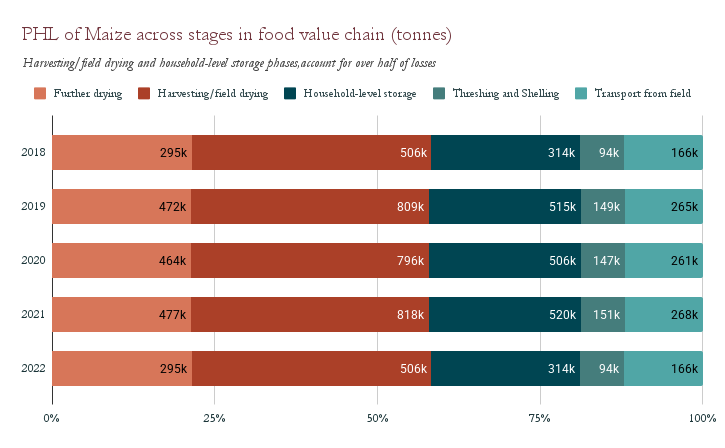
\includegraphics[scale=0.5]{Figures/phl_across_value_chain.png}
    \caption{\acrshort{phl} loss in the various steps in the maize value chain. Source: APHLIS database, 2019}
    \label{fig:figure-02}
\end{figure}

PHL is not just loss of food; it translates to loss in precious nutritional value. Maize for example is a staple food in Nigeria and PHL losses mean less nutrients for people. The data shows that, the amount of nutrients lost from PHL, equivalent to the average person's dietary requirements has been on the rise since the 2000s as \autoref{fig:figure-03} shows.

\begin{figure}[H]
    \centering
    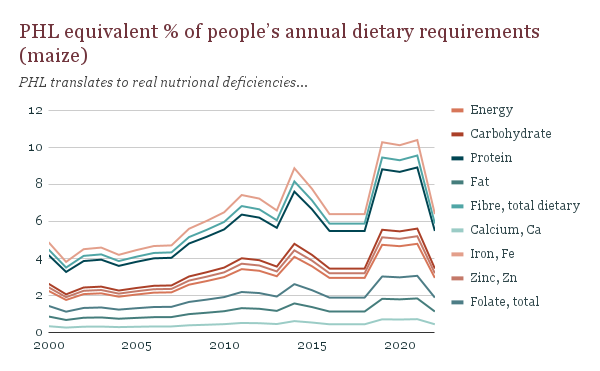
\includegraphics[scale=0.7]{Figures/phl_nutritional_maize.png}
    \caption{\acrshort{phl} expressed in the percentage of the average person's annual dietary requirements}
    \label{fig:figure-03}
\end{figure}


Analysis of \acrshort{phl} loss in maize in 2022 is summarised in \autoref{tab:table-01}. For instance, the post-harvest loss of approximately 4.8 trillion kcal of energy and 878 million kg of carbohydrate alone could have met the annual energy and carbohydrate requirements of over 5.7 million and 6.7 million people, respectively, across the total Nigerian population. These losses represent 2.9\% and 3.5\% of the total population's annual requirements for energy and carbohydrate. This is an obvious symptom of inefficiency in the food system that prevents available nutrients from reaching consumers.

The nutritional impact is particularly pronounced for vulnerable demographic groups, such as males aged 9-13 years. Within this focal group, the lost maize could have fulfilled the annual protein requirements for nearly 12.7 million individuals, a figure exceeding the total population of this demographic in 2022. This translates to a staggering 98.4\% of the focal group's annual protein needs that were not met due to post-harvest losses. 
% Similarly, the losses of essential micronutrients like Iron and Zinc also demonstrate critical impacts on this age group, representing 102.5\% and 46.3\% of their annual requirements, respectively. 
% While the lost quantities of some nutrients like Vitamin A and Vitamin C were negligible in maize for this period, the substantial losses of protein, iron, and zinc underscore how post-harvest issues directly exacerbate micronutrient deficiencies and food insecurity among vulnerable populations in Nigeria. 
% Addressing these losses is therefore critical not only for improving food availability but also for improving the nutritional status of the population, particularly among children and adolescents.
\begin{table}[h!]
    \centering
    \caption{Nutritional Impact of Maize Post-Harvest Losses in Nigeria, 2022}
    \label{tab:table-01}
    % Use tabularx with \textwidth for the total width
    % Define columns: l, r, and L for wrapping columns
    
    \begin{tabularx}{\textwidth}{|l|r|L|L|L|L|}
        \hline
        \multirow{2}{*}{Nutrient} & \multirow{2}{*}{Quantity lost postharvest} & \multicolumn{2}{c|}{Total population, Nigeria} & \multicolumn{2}{c|}{Male, 9-13 years, Nigeria} \\
        \cline{3-6}
         &  & Number of people's annual nutritional requirements lost & \% of population nutritional requirements lost & Number of people in focal group's annual nutrient requirements lost & \% of focal group population's annual nutritional requirements lost \\
        \hline
        Energy & 4,797,678,189 kcal & 5,771,644 & 2.9 & 5,752,439 & 44.7 \\
        Carbohydrate & 878,428,757 kg & 6,763,242 & 3.5 & 6,740,738 & 52.4 \\
        Protein & 126,471,746 kg & 10,744,369 & 5.5 & 12,664,398 & 98.4 \\
        Fat & 56,362,409 kg & 2,214,600 & 1.1 & 2,211,670 & 17.2 \\
        Fibre, total dietary & 133,345,210 kg & 11,522,627 & 5.9 & 11,420,111 & 88.8 \\
        Calcium, Ca & 261,192 kg & 864,988 & 0.442 & 650,540 & 5.1 \\
        Iron, Fe & 42,615 kg & 12,528,603 & 6.4 & 13,192,626 & 102.5 \\
        Zinc, Zn & 21,308 kg & 6,266,152 & 3.2 & 5,956,874 & 46.3 \\
        Folate, total & 357.4 kg & 3,686,759 & 1.9 & 3,916,933 & 30.4 \\
        Vitamin A (RAE) & 0 kg & 0 & 0 & 0 & 0 \\
        Vitamin C & 0 kg & 0 & 0 & 0 & 0 \\
        \hline
    \end{tabularx}
\end{table}

\acrshort{phl} also reflects as financial loss. Between 2013 and 2020, the financial impact of rice PHL grew from \$536,467,825 in 2013 to \$970,343,075 in 2020.

While the losses remained below 1\% of the national agricultural GDP, the rising absolute value calls for attention to mitigation strategies to alleviate the effects on farmer's income, availability of rice to consumers and overall economic stability.


\begin{figure}[H]
    \centering
    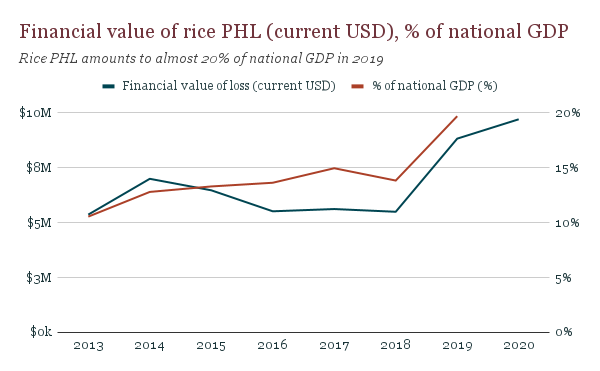
\includegraphics[scale=0.7]{Figures/phl_rice_financial_value.png}
    \caption{Financial value of rice PHL loss in Nigeria from 2013 to 2020. Source: APHLIS database, 2019}
    \label{fig:figure-04}
\end{figure}



\section{Impact on Youth and National Economy}

\acrshort{phl} have far-reaching consequences for Nigeria’s economy and youth engagement in agriculture. Economically, \acrshort{phl}  represents wasted farmer income and lost food value, with maize losses alone accounting for approximately 0.9\% of agricultural GDP. Furthermore, the inefficiency in food production results in under-utilized land—31\% of Nigeria’s cropland—and contributes to 5\% of the country’s greenhouse gas emissions. These losses inflate food prices, exacerbate food insecurity, and weaken national economic stability.

Beyond economic concerns, PHL directly affects Nigeria’s youth, the largest segment of the population. The agricultural sector, despite its substantial contribution to the GDP (around 24\%), is dealing with a dwindling workforce due to an aging farming population and the discouraging effects of post-harvest losses. Young people, who could drive innovation and modernization in agriculture, often view the sector as unappealing due to the visible waste and financial risks. Watching hard-earned produce deteriorate before reaching consumers discourages entrepreneurial efforts and limits agriculture’s potential as a viable career path.

Reducing post-harvest losses is therefore crucial to stabilizing the economy and making agriculture more attractive to younger generations. It would increase food availability without requiring expansion of farmland, improve farmers’ livelihoods, and foster a more resilient food system. Addressing PHL could encourage youth participation in agriculture, helping Nigeria move toward food self-sufficiency and boosting export potential. In essence, tackling post-harvest waste is not just about protecting farmers—it’s about securing Nigeria’s future.nd \(iv)\) designing it to be user-friendly, especially for newcomers.
}
\chapter[Causes Of PHL]{Contributory factors to \acrshort{phl} in Nigeria}
\label{cp:causes-of-phl}

{
\parindent0pt

%\textit{Authors: Edun Joshua, Mbuotidem Awak, Makinde Kayode}

% \textit{Current Version: 2.2.4}

%\textit{License: \LaTeX~Project Public License v1.3c}

%\textit{Official Repository: \href{https://github.com/joseareia/ipleiria-thesis}{GitHub Repository}}

\vspace{.935em}
 This chapter examines the primary factors driving Nigeria’s post-harvest losses – poor transportation infrastructure, inadequate storage and cold-chain capacity, and limited market access – and explains how each contributes to the problem.

 \section{Poor Transportation Infrastructure}
Nigeria’s road and transport network is widely cited as a major culprit in post-harvest loss. Most rural roads are unpaved and poorly maintained, making travel slow, costly, and unreliable \citep{PinnacleTimes2024, VoiceofNigeria2023}. In fact, about 80\% of Nigerian feeder roads are unpaved and become impassable during the rainy season \citep{PinnacleTimes2024}. This forces farmers to make long, bumpy trips to market on motorcycle or in old trucks. One maize farmer in Osun State lamented that after harvesting, “we have no means of transporting [products] to urban centres…we eat what we can while a good percentage wastes away” \citep{PinnacleTimes2024}.
\\

Bad roads and inadequate vehicles increase both transit time and physical damage to produce. Perishable crops (tomatoes, peppers, leafy vegetables) begin to spoil or get bruised during long journeys in hot, open trucks. In one reported case, a Kano tomato farmer drove 14 hours in a non–air-conditioned van on a 32°C day; by the time his produce reached market, the tomatoes were already “rotting” and often thrown away unsold \citep{Ikegwuonu2018}.
Such delays and heat stress can reduce shelf life from days to hours. Even for storable staples (maize, rice, yams), poor roads mean farmers often wait too long before selling; delays invite pests (weevils, rodents) and moisture damage during transport.
\\

This infrastructure gap has been quantified in national studies. For example, the Food and Agriculture Organization (FAO) estimates that up to 40\% of Nigeria’s agricultural output is lost post-harvest due to inadequate infrastructure \citep{PinnacleTimes2024}. Government officials also emphasize that improving rural roads can directly cut losses: according to Nigeria’s Rural Access Project coordinator, better feeder roads and bridge repairs would “reduce post-harvest losses, cost of transportation and accident rates” for farmers citep{VoiceofNigeria2023}.
\\

In short, the combination of long distances, rough roads and few refrigerated trucks means a large share of freshly-harvested crops never reach markets in good condition.

\subsection{Key effects of poor transportation}

\begin{description}
    \item[Delays and spoilage:] Long travel times on bad roads (often on footpaths or seasonal tracks) expose produce to heat, moisture and pests, so fruits and vegetables rot en route \citep{Ikegwuonu2018}.
    
    \item[Physical damage] Bumpy rides in unpadded vehicles bruise grains and produce, leading to quality losses. Crushed bags attract pests and mold.
    
    \item[High costs and leakage] Weak logistics force farmers to pay steep transport fees, effectively shrinking their margins. Some give up on distant markets altogether, dumping excess harvest near the farm.
\end{description}


Together, these factors mean that many Nigerian farmers see double-digit percentage losses just due to transit. For instance, data from the African Postharvest Losses Information System (APHLIS) shows ~17\% of Nigeria's maize is lost from harvest through delivery \citet{APHLIS}- and that figure would be higher on poor roads.


\subsection{Inadequate Cold Storage and Processing}
Another root cause of Nigeria’s post-harvest losses is the near-absence of cold-chain and storage facilities. Most Nigerian farmers and traders have no access to refrigerated warehouses or cooling trucks. After harvest, highly perishable goods like tomatoes, fruits, vegetables, dairy and meat immediately begin to deteriorate without temperature control \citep{OTACCWA2025}.
\vspace{\myvspace}

Nigeria’s climate and power constraints make this especially severe. In most rural areas, electricity is intermittent or unavailable, and conventional refrigerators require too much power. As one report notes, “unlike the United States and Europe…cold refrigeration is virtually nonexistent in [Nigerian] farms and marketplaces” \citep{Ikegwuonu2018}.
\vspace{\myvspace}

The impact is dramatic: one analysis found that about 45\% of Nigeria’s perishable produce spoils at some point after harvest solely because of lack of cold storage\citep{Ikegwuonu2018}. Without refrigeration, simple transport times of a day or two can be fatal. For example, in the IFPRI ColdHubs case study above, tomatoes lost roughly two-thirds of their market value by afternoon due to heat and rot \citep{Ikegwuonu2018}. Similarly, fruits like mangoes or watermelons will ferment or shrivel if not cooled within hours. Even root crops (cassava, yams) and grains lose quality if stored too long without drying or cooling; high humidity in sacks leads to mold and aflatoxins.
\vspace{\myvspace}

Moreover, Nigeria lacks processing and value-addition facilities that could reduce spoilage. For instance, small-scale drying kilns, canning plants, or flour mills are rare in many regions. If farmers had accessible rice mills or tomato canneries nearby, they could convert part of their harvest to shelf-stable products, greatly extending shelf life. In reality, most produce must be sold raw. This mismatch means that whenever markets glutted after harvest, farmers often have no choice but to sell quickly at low prices or waste the excess.
\vspace{\myvspace}

In sum, the lack of a modern cold chain (from farm to market) means Nigeria forfeits nearly half its high-value harvest to heat and spoilage
\citep{Ikegwuonu2018, OTACCWA2025}. Experts note that “a modern cold chain system, combined with improved infrastructure and logistics, will be key to mitigating these losses” \citep{Ikegwuonu2018, OTACCWA2025}. As it stands, perishables often never reach peak freshness, and farmers’ incomes suffer accordingly.

\subsection{Limited Market Access and Information}
A related factor is how market barriers amplify post-harvest losses. Many smallholder farmers in Nigeria are geographically or socially isolated from buyers. Poor linkages mean harvests cannot be sold quickly and efficiently. Key issues include:

\begin{description}
\item[Fragmented production:] Nigerian farms are small and scattered. Most farmers sell independently in local village markets. Without aggregation, they face high transaction costs transporting small loads, and cannot negotiate strong prices. The \citet{FarmSupportSolutions2025} notes that fragmented production and inconsistent quality “reduces market acceptance” and makes rural supply chains inefficient. When multiple small producers simultaneously bring the same crop to town, local prices crash and some output cannot be sold at all.

\item[Lack of price and demand information:] Many farmers do not have real-time data on market prices or demand trends. Without mobile market services or cooperatives, they often sell based on gut feeling. This information gap means farmers miss opportunities to time their sales for higher prices or send produce where demand is growing. In practice, it leads to gluts in some markets (driving prices down and unsold stacks to waste) while other regions suffer shortages. As FSSS reports, “limited market information…leads to low economies of scale” and exacerbates waste \citep{FarmSupportSolutions2025}.

\item[Inefficient value chains:] Poor market access also results from missing infrastructure and services. For example, contract storage (warehouse receipt systems) or cold trucks for linking farmers to distant processors are largely unavailable. Without these, farmers often face long waits or forced distress sales. Research in Nigeria has noted that inadequate marketing systems and governance gaps in distribution (such as lack of financing for storage) are key socio-economic causes of loss \citep{Ogundele2022}.
\end{description}

In other words, even if crops survive transport, market inefficiencies can leave them unsold. For instance, one survey found that almost half of smallholder farmers were unable to sell their preferred quantity because of volatile prices and a lack of buyers
\vspace{\myvspace}

Addressing market access could dramatically cut losses: digital marketplaces and aggregation hubs are emerging as solutions. By connecting farmers directly with buyers and sharing price information, such platforms reduce the risk of unsold crop. For example, pilot programs like Foodstuff Store and Soluta leverage mobile apps to link remote farmers with city consumers and traders, helping ensure produce finds a market quickly \citep{Tenebe2024, FarmSupportSolutions2025}. These innovations hint at how improved market linkages can complement transport and storage solutions.

\subsection{Conclusion}

Nigeria’s high post-harvest losses have clear, practical causes rooted in infrastructure and market systems. In summary: crumbling rural roads and transport mean crops spoil before sale
\citep{PinnacleTimes2024, VoiceofNigeria2023}
; absence of cold storage and processing leaves perishables to rot or shrivel
\citep{Ikegwuonu2018, OTACCWA2025}
; and poor market integration forces farmers into inefficient, wasteful sales patterns
\citep{FarmSupportSolutions2025}. These problems are interlinked: for example, even if transport is available, the benefit is lost if there is nowhere to store or sell the produce at proper prices. Studies emphasize that tackling Nigeria’s PHL requires a multifaceted approach. The challenges are “complex and interrelated,” so solutions must combine technical fixes with economic and policy reforms
\citep{Ikegwuonu2018, Abulude2024}.
\vspace{\myvspace}

In practice, this means investing in all links of the chain: paving and maintaining feeder roads and bridges, expanding clean energy for cold storage, supporting local processing centers, and empowering farmers with market data and aggregation mechanisms. According to experts, “a modern cold chain system, combined with improved infrastructure and logistics, will be key to mitigating these losses”\citep{Ikegwuonu2018}.
\vspace{\myvspace}

In conclusion, reducing Nigeria’s PHL burden (currently on the order of tens of billions of naira per year) hinges on strengthening the transportation-storage-market triad. Hackathon innovations that create digital marketplaces or logistics solutions directly address this nexus. By helping farmers find buyers and manage their produce more efficiently, such tools can cut waste and preserve value. In doing so, they support food security and farmers’ incomes – goals that depend squarely on fixing the infrastructure and informational gaps highlighted above.
}
\chapter[Okra: Our Solution Proposal]{Okra: Our Solution Proposal}
\label{cp:okra-solution}

{
\parindent0pt

\section{Core Concept and Functionality}
Okra is a mobile-first, web-enabled platform designed as a comprehensive ecosystem to mitigate PHL. The platform serves three primary user groups:

\begin{description}
    \item[Farmers/Producers:] Can create profiles, list their produce (crop type, quantity, harvest date, location), upload images for AI assessment, set indicative prices, and view market demand.
    
    \item[Buyers] Can search for specific produce based on type, quantity, quality (informed by AI score), and location. They can connect with farmers, negotiate, and arrange purchases. Buyers include wholesalers, retailers, processors, and direct consumers.
    
    \item[Logistics Providers] Can register their services (vehicle type – including refrigerated options, capacity, operational routes, pricing). The platform facilitates matching them with farmers/buyers needing transport.
\end{description}

\subsection{Marketplace Networking}
Farmers and producer groups register on the app to list available produce (crop type, quantity, harvest date). Buyers – including wholesalers, processors, and retailers – can search and place orders by region and crop. By centralizing listings, the app ensures farmers find customers quickly, and buyers can discover sources of fresh produce. This reduces unsold inventory and match supply to demand in real time.

\subsection{Logistics Integration}
The app includes a dashboard for logistics providers (truckers, couriers, cold-chain operators). When a sale is made, the system can automatically offer transport jobs to verified drivers. Users can see available vehicles, rates, and track shipments. For example, a farmer in Kano could schedule a refrigerated truck to deliver tomatoes to Lagos. This ensures reliable transport capacity and route planning, cutting delays that lead to spoilage.

\subsection{AI-Powered Insights}
A novel AI feature uses computer vision to analyze produce quality. Farmers or cooperatives upload smartphone images of their harvest batches. The app’s AI model assesses freshness (e.g. spotting bruises, mold, color) and estimates volume or weight from the images. This accomplishes two goals: (1) It provides an objective quality grade for buyers to see, increasing trust. (2) It forecasts how long the produce will remain saleable. The model improves over time as more labeled images are fed back, refining its predictions.

\subsection{Youth-led Agribusiness Empowerment}
The platform encourages youth entrepreneurship. For example, tech-skilled youth can be trained to help digitize farms (taking images, using the app), to become last-mile delivery drivers, or to manage aggregation hubs. The platform could partner with agricultural colleges or startup incubators to recruit graduates. By framing agriculture as a tech-enabled business, the app draws young people into value chains. In effect, it transforms farming from subsistence into a connected, data-driven marketplace, which is more attractive to the next generation.

\begin{block}[note]
    \textit{Because of the time span of the hackathon, development of Okra is not complete. Part of the frontend and most of the backend are still in development. The following sections show the current state of the project, including the mockups and the data strategy.}
    \end{block}


\section{Screens}


\begin{figure}[H]
    \centering
    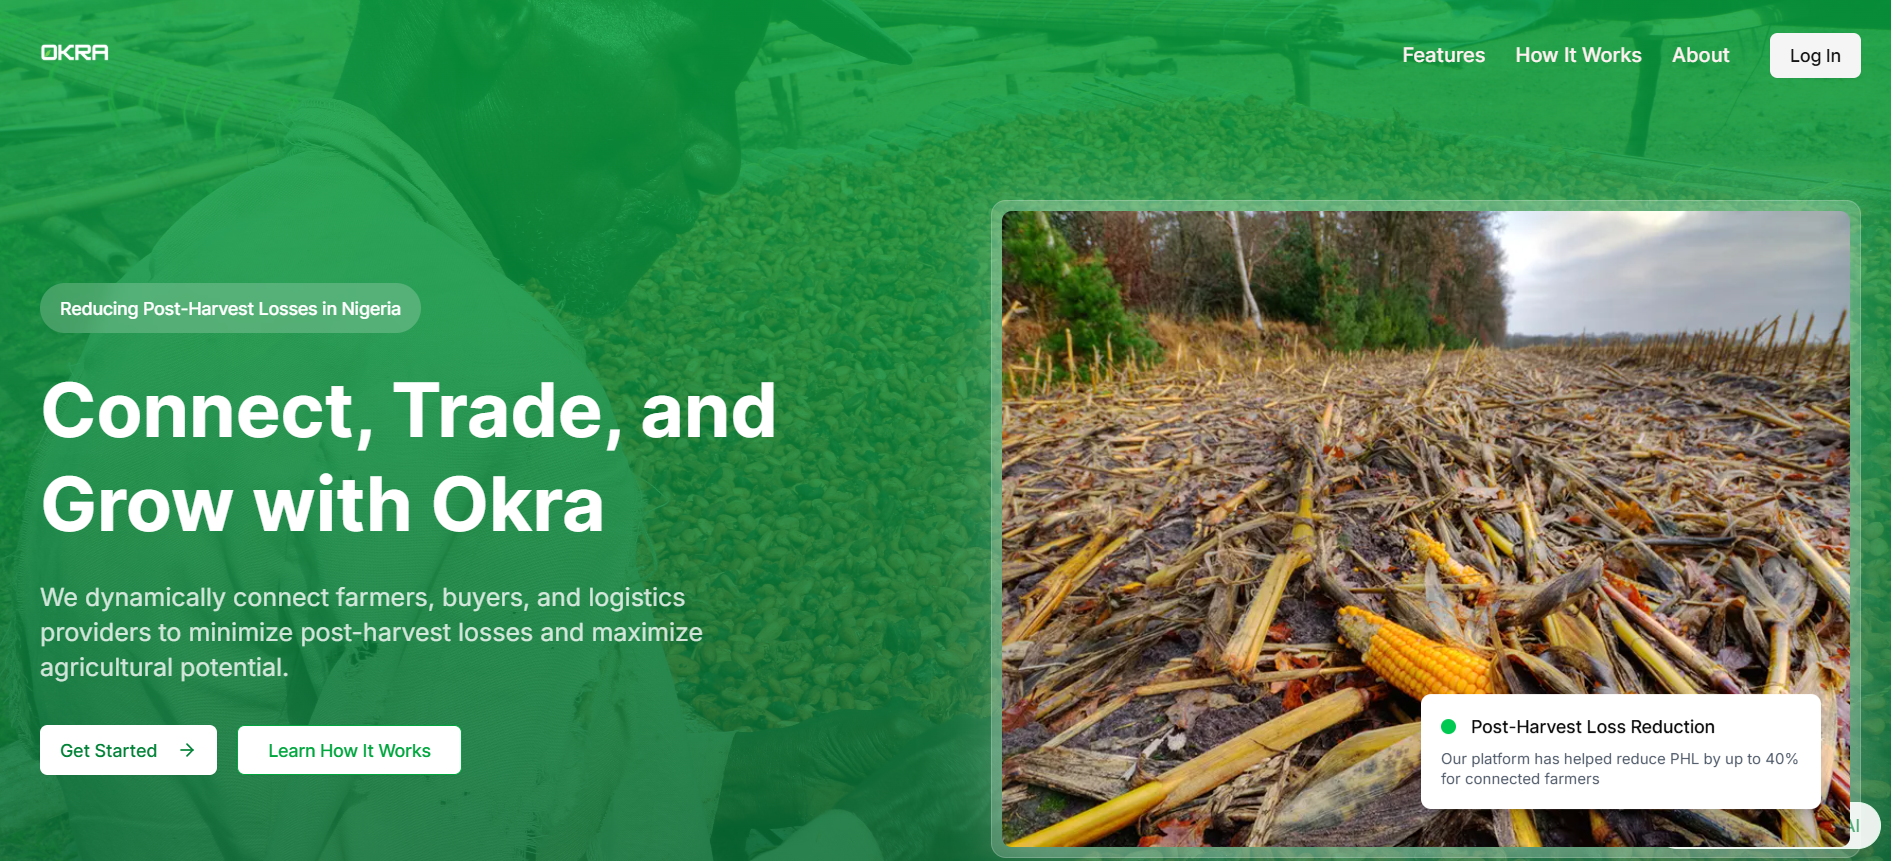
\includegraphics[scale=0.3]{Figures/okra_mockup_landing.png}
    \caption{Screenshot of the landing page}
    \label{fig:figure-05}
\end{figure}


\begin{figure}[H]
    \centering
    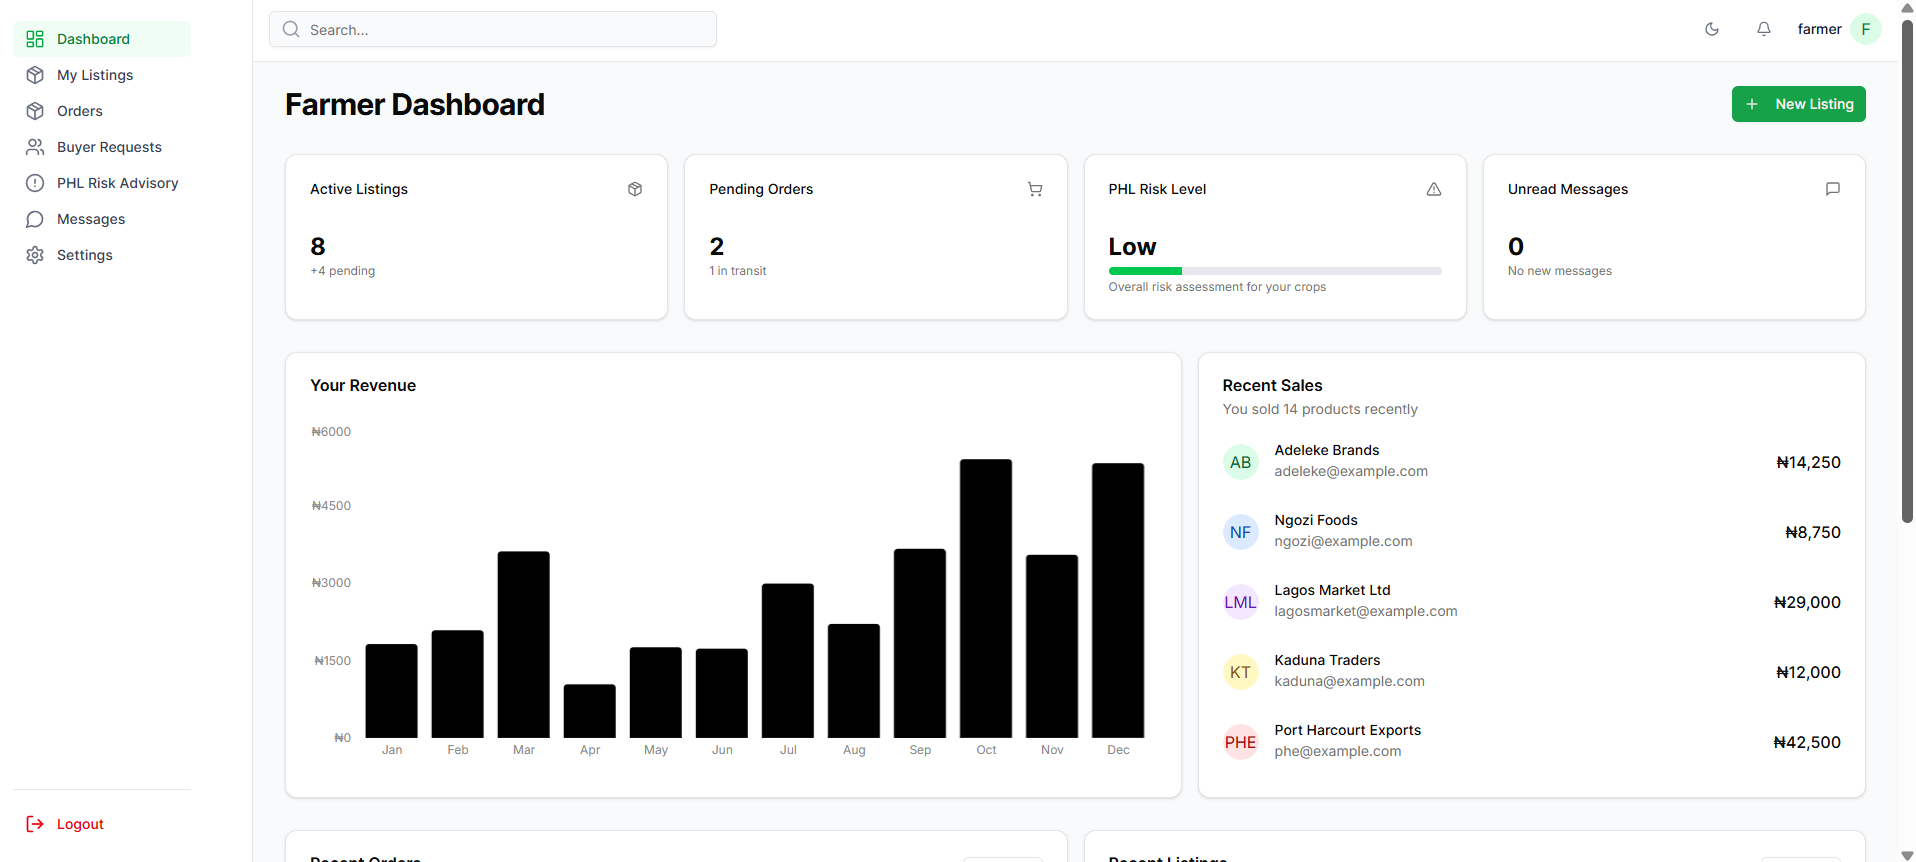
\includegraphics[scale=0.3]{Figures/okra_mockup_farmer_db.png}
    \caption{Screenshot of the farmer's dashboard}
    \label{fig:figure-06}
\end{figure}


\begin{figure}[H]
    \centering
    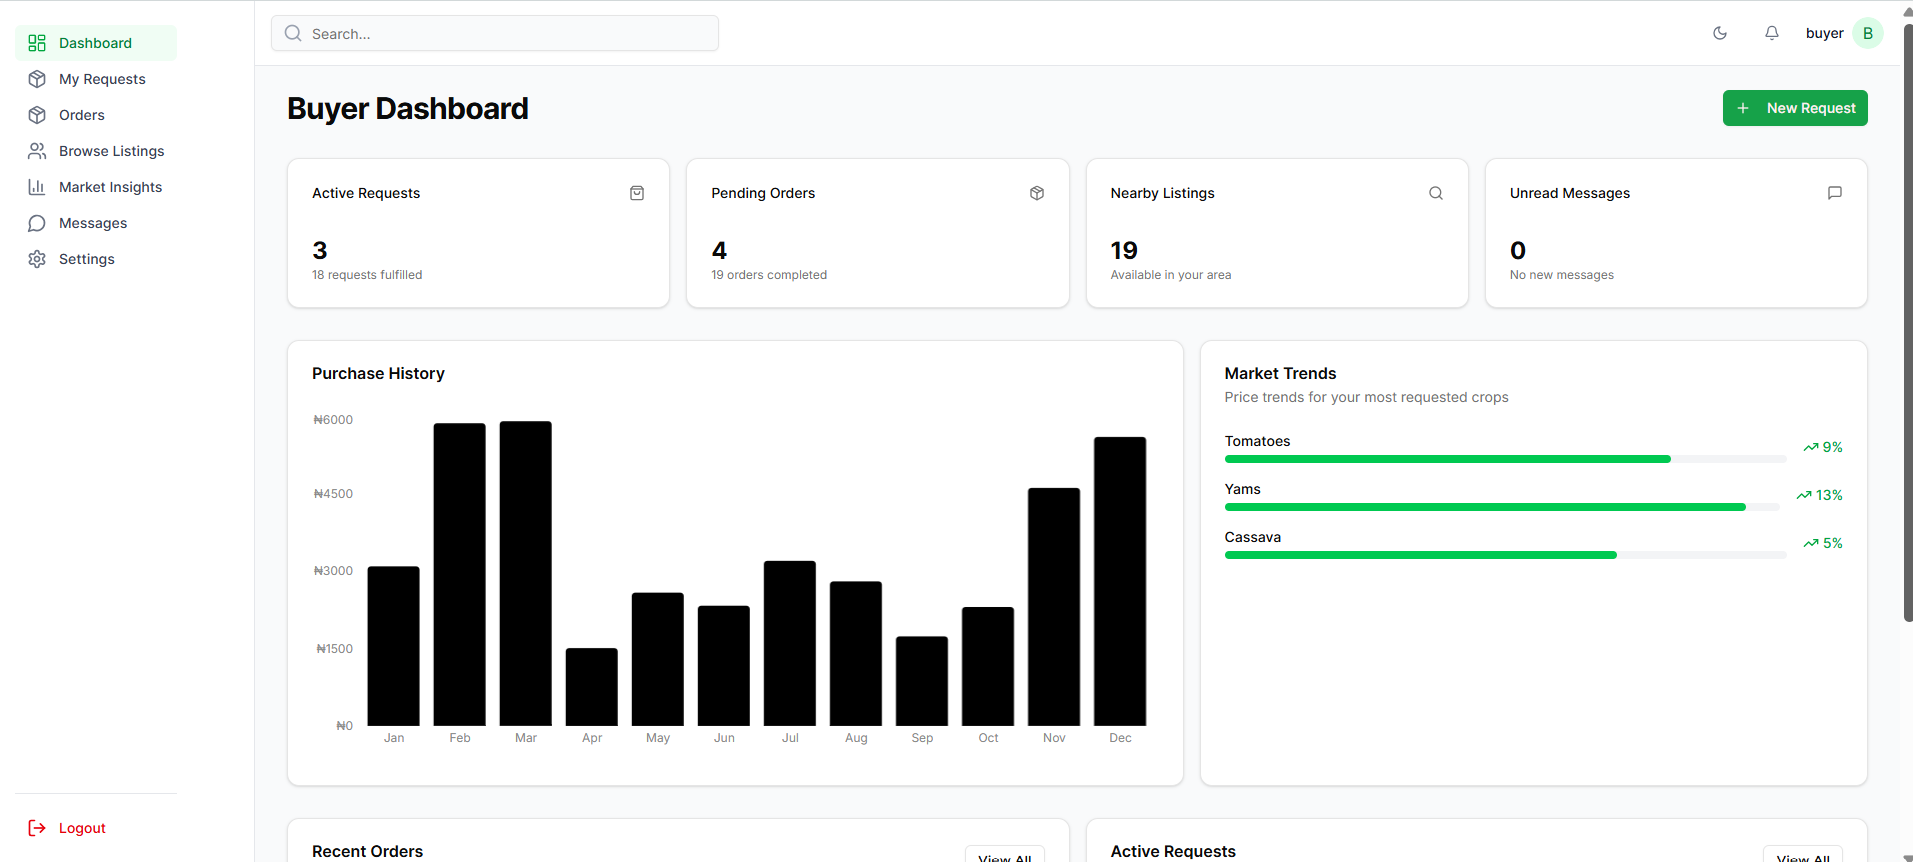
\includegraphics[scale=0.3]{Figures/okra_mockup_buyer_db.png}
    \caption{Screenshot of the buyers's dashboard}
    \label{fig:figure-07}
\end{figure}

\begin{figure}[H]
    \centering
    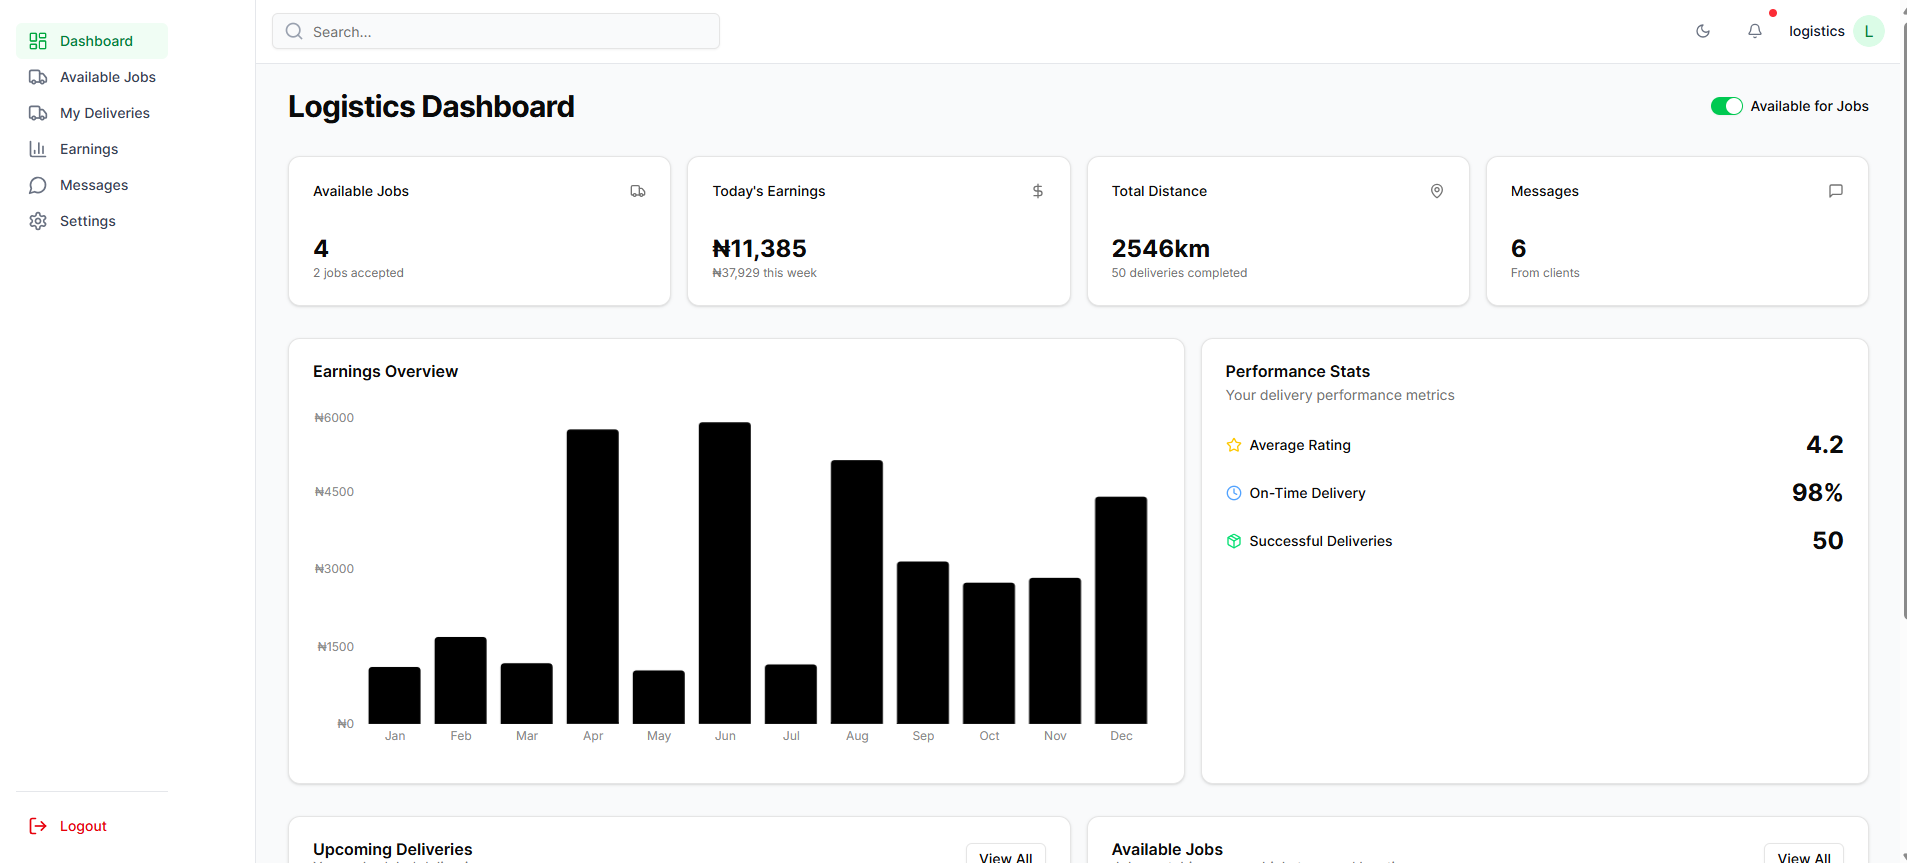
\includegraphics[scale=0.3]{Figures/okra_mockup_logistics_db.png}
    \caption{Screenshot of the buyers's dashboard}
    \label{fig:figure-08}
\end{figure}


\section{Data Strategy}

\subsection{Image Data Collection}
We will collect large numbers of labeled images of harvested produce. This will be done in phases: initially, a pilot program in a few regions (e.g. Kano for tomatoes, Adamawa for maize) will train extension agents and youth volunteers to photograph produce at harvest and at sale. Each image will be tagged with metadata (crop type, variety, region, time, moisture, storage conditions, etc.). Over time, farmers using the app will also upload photos for every batch they list, creating a growing dataset.

\subsection{Data Labeling and Training}
Using expert agronomists and community training, images will be labeled for freshness (e.g. “Fresh”, “Moderately aged”, “Spoiled”) and total count/weight. This labelled dataset feeds the computer vision model. We will employ transfer learning on convolutional neural networks so the AI can accurately assess new images it has not seen before. The initial model will be tested for accuracy and iteratively improved as more data arrives.

\subsection{Feedback Loop (Active Learning)}
Post-deployment, the app will track outcomes of predicted vs. actual. For example, if the AI predicts 10 days of shelf life but spoilage occurs in 7 days, this discrepancy is logged. Buyers and farmers can rate or report the accuracy of freshness ratings. This feedback is used to retrain the model periodically, increasing its accuracy over time. In effect, the app learns from real-world results.

\section{Auxiliary data sources}
In addition to user-generated data, the system will integrate public and commercial datasets for context. Possible sources include:


\begin{description}
    \item[Crop statistics:]  Government or FAO data on regional production volumes and seasonality for major crops.
    
    \item[Geolocation] Maps of farm locations, major roads, market centers.
    
    \item[Weather/Climate] Historical and current weather data per region, since humidity and temperature affect spoilage.
    \item[Market Prices]  Data from local commodity exchanges or market surveys, to show price trends.
    \item[Demographic Data] Farm population and sizes, to profile areas served.This external data enriches the dashboard: for instance, linking rainfall patterns to losses in maize, or highlighting regions that produce a given crop. All data is tied to time and location, enabling spatio-temporal analysis.
\end{description}

\subsection{Privacy and Governance}
Farmers’ personal data (names, exact addresses) will be protected. Only aggregate or anonymized data used on dashboards. Data use agreements will ensure that insights (e.g. “X tonnes of tomatoes sold from Kano”) respect user privacy while guiding decisions.




Geolocation: Maps of farm locations, major roads, market centers.
Weather/Climate: Historical and current weather data per region, since humidity and temperature affect spoilage.
Market Prices: Data from local commodity exchanges or market surveys, to show price trends.
Demographic Data: Farm population and sizes, to profile areas served.
This external data enriches the dashboard: for instance, linking rainfall patterns to losses in maize, or highlighting regions that produce a given crop. All data is tied to time and location, enabling spatio-temporal analysis.
Privacy and Governance: Farmers’ personal data (names, exact addresses) will be protected. Only aggregate or anonymized data used on dashboards. Data use agreements will ensure that insights (e.g. “X tonnes of tomatoes sold from Kano”) respect user privacy while guiding decisions.

}

%%% Bibliography %%%
\renewcommand{\refname}{Bibliography}
\printbibliography[title={\refname},heading=bibintoc]

%%% Appendices: Work that *YOU* Developed %%%
% \appendix
% \ifthenelse{\equal{\LanguageOption}{portuguese}}{
    \addtocontents{toc}{\protect\contentsline{chapter}{Apêndices}{}{}}
}{
    \addtocontents{toc}{\protect\contentsline{chapter}{Appendices}{}{}}
}

\ifthenelse{\equal{\MediaOption}{paper}}{\blankpage}{\clearpage}
\begin{center}
    \crimsonfont
    \thispagestyle{empty}
        
    \vspace*{\fill}
    \ifthenelse{\equal{\LanguageOption}{portuguese}}{%
        {\LARGE\fontsize{26}{26}\selectfont\textcolor{maincolor}{Apêndices}\par}
    }{%
        {\LARGE\fontsize{26}{26}\selectfont\textcolor{maincolor}{Appendices}\par}
    }
    \vspace*{\fill}
\end{center}
\MediaOptionLogicBlank
% \chapter{Showcasing the First Appendix}
\guideinfo{Appendices contain supplementary material \textbf{created by the author} that enhances the reader’s understanding of the dissertation while not being essential for following the primary narrative. These sections often include detailed tables, figures, complex calculations, or materials like survey questions and interview transcripts produced in the course of the research. The appendices allow readers to explore the research in greater detail, offering a deeper insight into methods and findings without interrupting the main body of work.}
% % Recommended dimensions for a landscape layout; adjust as needed.
\begin{landscapemode}{297mm}{420mm}
    \chapter{Showcasing the Second Appendix}
    \blindtext[5]
\end{landscapemode}

% %%% Annexes: Work that *YOU DID NOT* Develop %%%
% \ifthenelse{\equal{\LanguageOption}{portuguese}}{
    \addtocontents{toc}{\protect\contentsline{chapter}{Anexos}{}{}}
}{
    \addtocontents{toc}{\protect\contentsline{chapter}{Annexes}{}{}}
}

\setcounter{chapter}{11} % To start at the "L" chapter.
\MediaOptionLogicAnnexes
\begin{center}
    \crimsonfont
    \thispagestyle{empty}
        
    \vspace*{\fill}
    \ifthenelse{\equal{\LanguageOption}{portuguese}}{%
        {\LARGE\fontsize{26}{26}\selectfont\textcolor{maincolor}{Anexos}\par}
    }{%
        {\LARGE\fontsize{26}{26}\selectfont\textcolor{maincolor}{Annexes}\par}
    }
    \vspace*{\fill}
\end{center}
\MediaOptionLogicBlank
% \chapter{Showcasing the First Annex}
\guideinfo{Annexes are supplementary sections in a dissertation that provide additional information or external documents not essential to the main arguments but that support or complement the research. Unlike appendices, \textbf{annexes generally contain material that was not developed by the author}, such as reports, legal documents, or published datasets from external sources. This information is placed separately to keep the main content concise, allowing readers access to relevant external references without disrupting the dissertation's flow.}

%%% Back Page %%%
\ifthenelse{\equal{\MediaOption}{paper}}{\blankpage}{}

\clearpage
\null
\thispagestyle{empty}

\ifthenelse{\equal{\CoverOption}{classic}}{
    \newcommand\BackgroundPicBackPage{%
    \put(0,0){%
    \parbox[b][\paperheight]{\paperwidth}{%
    \vfill
    \centering
    
\includegraphics[width=\paperwidth,height=\paperheight,keepaspectratio]{Figures/Theme/Back-Page-BG.pdf}%
    \vfill
    }}}
}{
    \newcommand\BackgroundPicBackPage{%
    \put(0,0){%
    \parbox[b][\paperheight]{\paperwidth}{%
    \vfill
    \centering
    
\includegraphics[width=\paperwidth,height=\paperheight,keepaspectratio]{Figures/Theme/Back-Page-BG-W.pdf}%
    \vfill
    }}}
}

\AddToShipoutPictureBG*{\BackgroundPicBackPage}

\newgeometry{margin=1.98cm, top=1.47cm, bottom=1.47cm}
\noindent\clearpage
\restoregeometry

\end{document}